To keep investigating the qualitative transformation in the dynamic patterns of the SDEs, the authors conducted another simulation, this time keeping the transmission rate under varying degrees of environmental perturbation in system \ref{eq:System3}. However they claim that, due to the significant impact of environmental perturbation on the model dynamics of RSV, they limited the perturbation range to a smaller extent compared to that of the birth rate shown in the previous simulations as we can see in Figure \ref{transmission1}.

\begin{figure}[h!]
    \centering
    \begin{subfigure}{0.4\textwidth}
        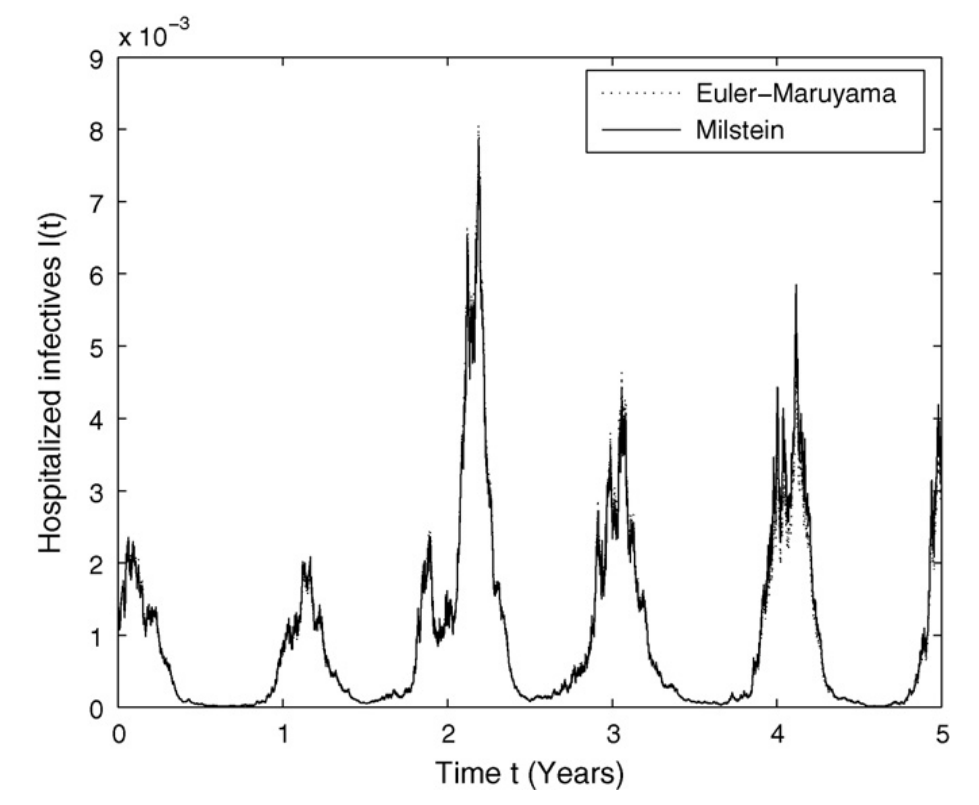
\includegraphics[width=\linewidth]{IMG/stoc_transmission_rate_perturbated.png}
        \caption{}
    \end{subfigure}
    \begin{subfigure}{0.4\textwidth}
        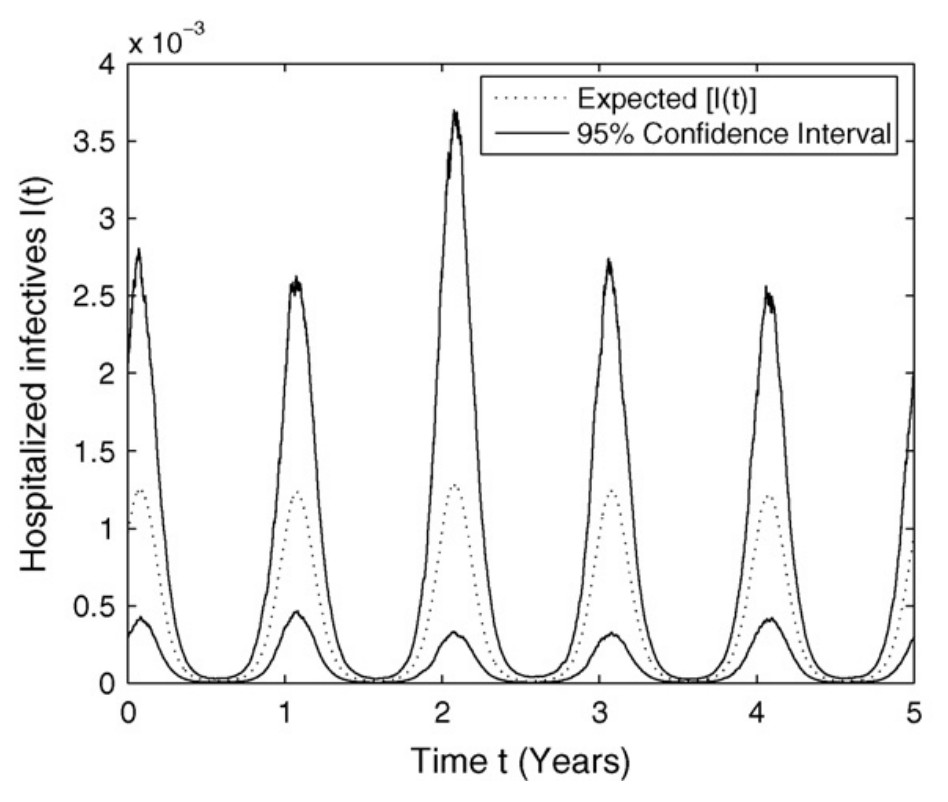
\includegraphics[width=\linewidth]{IMG/trasmisision_confidence1.png}
        \caption{}
    \end{subfigure}
    \caption{(a)Comparison between the Milstein and Euler-Maruyama stochastic scheme in regard to the infected sub population I(t) over a single simulation with transmission rate perturbation of 5\%.
    (b)Confidence intervals and expected behavior for the infected sub population I(t) when the RSV baseline transmission rate is perturbed of 1\%}
    \label{transmission1}
\end{figure}

Our implementation of the simulation shows a similar behaviour in Figure \ref{transmission2}. We can notice how in the span of ours ten simulation we can clearly see the stochasticity of the system, as our simulations are confined in the confidence interval delineated by the authors. This perturbation moves the system far away from the deterministic model and the birth perturbation model showing how the dynamics of infected population I(t) is greatly modified in response to such a small perturbation of 1\% and 2\%.

\begin{figure}[h!]
  \centering
  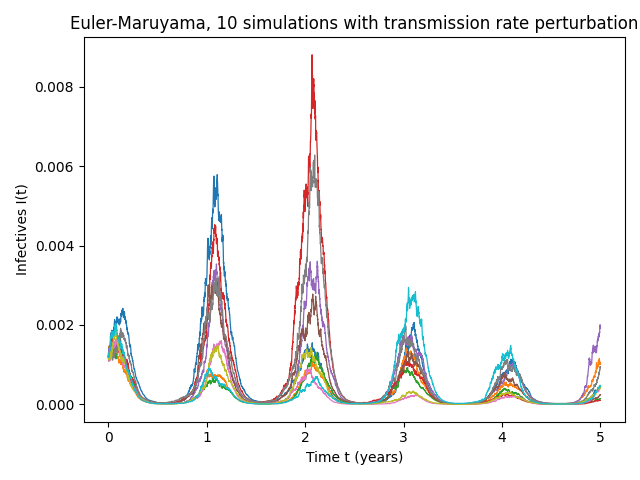
\includegraphics[width=0.8\textwidth]{IMG/transmission_aphabig_I(t).png}
  \caption{Euler-Maruyama stochastic schemes in regard to the infected sub population I(t) over multiple simulations with transmission rate perturbation at 2\% ($\alpha$ = 0.728).}
  \label{transmission2}
\end{figure}

Through the same simulations, they also computed the confidence intervals for each sub population within the stochastic system. They notice how the recovered R(t) and susceptible S(t), shown in Figure \ref{transmission3}, are expressing a peculiar behaviour.
\begin{figure}[h!]
    \centering
    \begin{subfigure}{0.4\textwidth}
        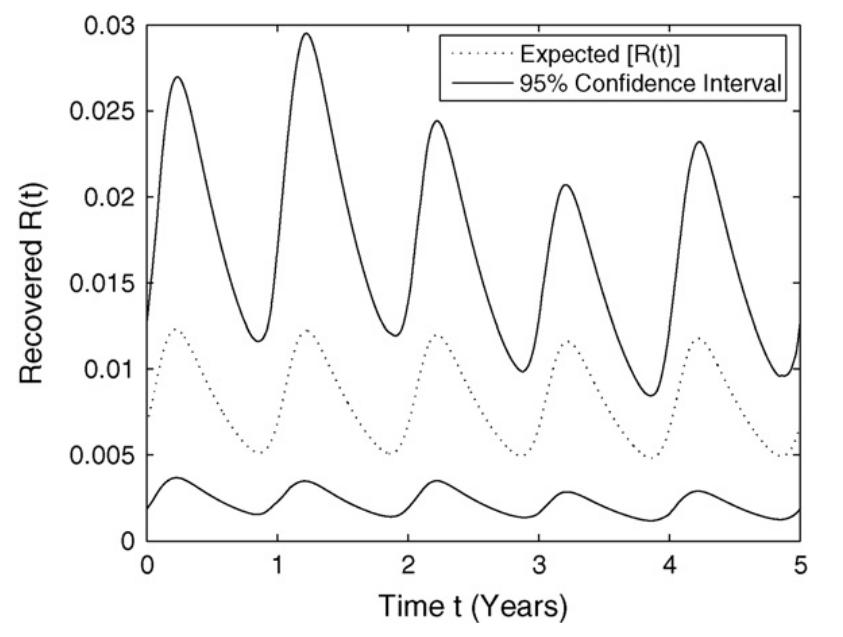
\includegraphics[width=\linewidth]{IMG/recovered_R(t).png}
        \caption{}
    \end{subfigure}
    \begin{subfigure}{0.4\textwidth}
        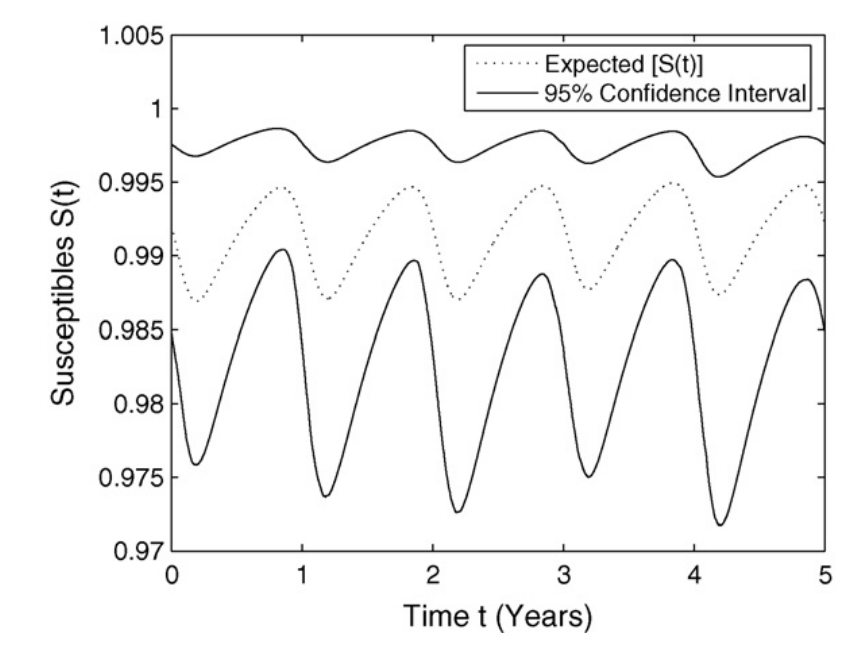
\includegraphics[width=\linewidth]{IMG/susceptible_S(t).png}
        \caption{}
    \end{subfigure}
    \caption{Confidence intervals and expected behavior for the recovered R(t)(a) and susceptible S(t)(b) sub populations, when the RSV baseline transmission rate is perturbed.}
    \label{transmission3}
\end{figure}
The degree of variation in the R(t) and S(t) sub populations, amplifies with an escalation in transmission rate perturbation. This intensification occurs even though the SDEs governing the two variables do not explicitly include a noisy seasonally forced cosinusoidal functions. Our results in Figure \ref{transmission4} conform with the simulations of the article. 

\begin{figure}[h!]
    \centering
    \begin{subfigure}{0.4\textwidth}
        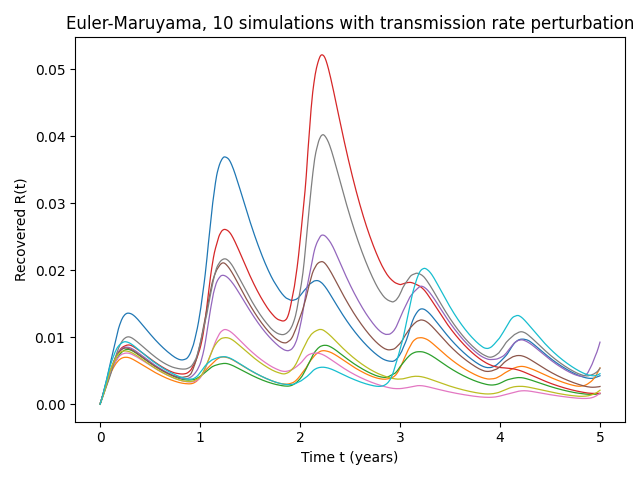
\includegraphics[width=\linewidth]{IMG/transmission_aphabig_R(t).png}
        \caption{}
    \end{subfigure}
    \begin{subfigure}{0.5\textwidth}
        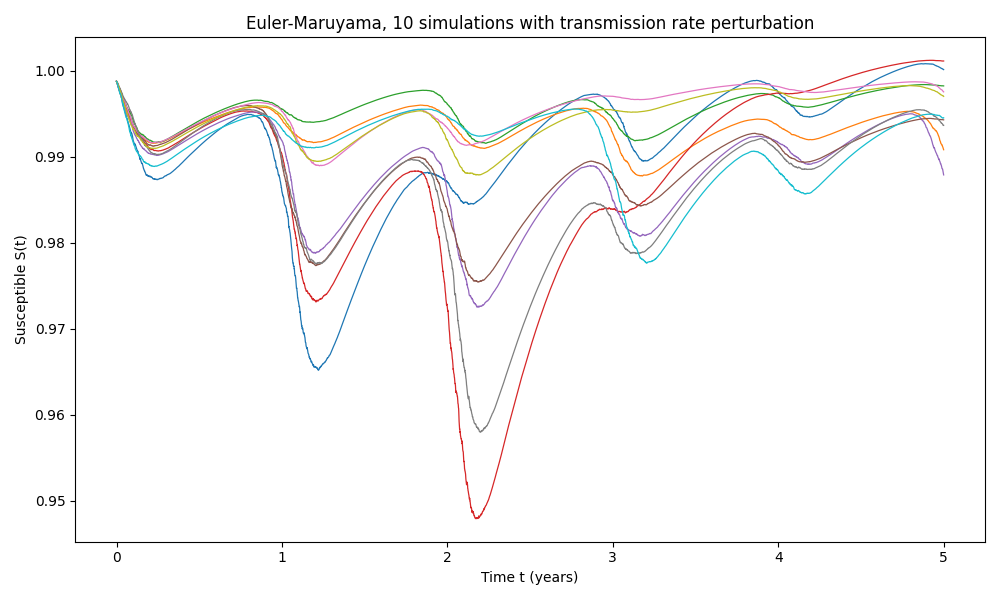
\includegraphics[width=\linewidth]{IMG/transmission_aphabig_S(t).png}
        \caption{}
    \end{subfigure}
    \caption{Euler-Maruyama stochastic graphs of recovered R(t)(a) and susceptible S(t)(b) sub populations over multiple simulations with transmission rate perturbation.}
    \label{transmission4}
\end{figure}

We can observe that, the introduction of a noise term in the equations produces an impact that allows the expression of the fundamental oscillatory nature of those sub populations.
\newpage